\chapter{Introductory Topics}

\section{An Introduction to Numerical Analysis}
\begin{quote}
    ``In the 1950s and 1960s, the founding fathers of [Numerical Analysis] discovered that
    inexact arithmetic can be a source of danger, causing errors in results that `ought'
    to be right.'' \\
    \\ Lloyd N. Trefethen (2006)
\end{quote}

The field of Numerical Analysis is really the study of how to take
mathematical problems and perform them efficiently and accurately on a computer.  There
are some problems where numerical analysis doesn't make much sense (e.g. finding an
algebraic derivative of a function) but for many problems a numerical method that gives an
approximate answer is both more efficient and more versatile than any analytic technique.
For example, if we needed to solve the differential equation $\frac{dy}{dt} = \sin(y^2) +
t$ the nonlinear nature of the problem makes it hard to work with analytically but
computational methods that result in a plot of an approximate solution can be made very
quickly and likely give enough of a solution to be usable.  Similarly, efficient
algorithms to do the basic operations of linear algebra (e.g. Gaussian elimination, matrix
factorization, or eigenvalue decomposition) are highly sought after and useful when
the matrices used for a model are very large. 

In this chapter we will discuss some of the basic underlying ideas behind the scenes in
Numerical Analysis, and the essence of the  above quote will be part of the focus of this chapter.
Particularly, we need to know how a computer stores numbers and when that storage can get
us into trouble.  On a more mathematical side, we offer a brief review of the Taylor
Series in this chapter. The Taylor Series underpins many of our approximation methods in
this class; so much so that we could easily rename the course: {\it Applied Taylor
Series}.  Finally, at the end of this chapter we provide several coding exercises that
will help you to develop your programming skills.  It is expected that you know some of
the basics of MATLAB programming before beginning this class.  If you need to review the
basics then see the Scientific Computing with MATLAB text cited in the bibliography of
these notes \cite{SciCompMATLAB}.  Trust me, you'll have more
than just the basics by the end.

\begin{center}
    Let's begin.
\end{center}
\section{Base 2 and Binary Arithmetic}
\begin{problem}\label{prob:base_10_faila}
    By hand (no computers!) compute the first 50 terms of this sequence with the initial condition $x_0 = 1/10$.
    \[ x_{n+1} = \left\{ \begin{array}{ll} 2x_n, & x_n \in [0,\frac{1}{2}] \\ 2x_n - 1, & x_n \in (\frac{1}{2},1] \end{array} \right. \]
    \end{problem}
\solution{
\[ x_n = \{1/10, 2/10, 4/10, 8/10, 6/10, 2/10, 4/10, 8/10, 6/10, \ldots \} \]
}

\begin{problem}\label{prob:base_10_failb}
Now use Excel and MATLAB to do the computations.  Do you get the same answers?  
\end{problem}
\solution{
In both Excel and MATLAB you lose accuracy at about the 40th iteration. 
}

\begin{problem}\label{prob:base_10_failc}
It seems like the computer has failed you!   What do you think happened on the computer
and why did it give you a different answer?  What, do you suppose, is the cautionary tale hiding behind the scenes with this problem?
\end{problem}
\solution{
The simplest answer is that $1/10$ is not computer representable.
}

\begin{problem}
    Now what happens with this problem when you start with $x_0 = 1/8$?  Why does this new
    initial condition work better?
\end{problem}

A computer circuit knows two states: on and off.  As such, anything saved in computer
memory is stored using base-2 numbers.  This is called a binary number system.  To fully
understand a binary number system it is worth while to pause and reflect on our base-10
number system for a few moments. 

What do the digits in the number ``$735$'' really mean?  The position of each digit tells
us something particular about the magnitude of the overall number.  The number $735$ can
be represented as a sum of powers of $10$ as
\[ 735 = 700 + 30 + 5 =  7 \times 10^2 + 3 \times 10^1 + 5 \times 10^0 \]
and we can read this number as $7$ hundreds, $3$ tens, and $5$ ones.
As you can see, in a ``positional number system'' such as our base-10 system, the
position of the number indicates the power of the base, and the value of the digit itself
tells you the multiplier of that power.  This is contrary to number systems like Roman
Numerals where the symbols themselves give us the number, and meaning of the position is
somewhat flexible.
% In other words, the location of the digit (as read from the right-hand side of the number
% starting at 0) is the power on the base, 10.  Similarly
The number ``48,329'' can therefore be interpreted as
\[ 48,329 = 40,000 + 8,000 + 300 + 20 + 9 = 4 \times 10^4 + 8 \times 10^3 + 3 \times 10^2 + 2
\times 10^1 + 9 \times 10^0, \]
Four ten thousands, eight thousands, three hundreds, two tens, and nine ones.

Now let's switch to the number system used by computers: the binary number system.  In a
binary number system the base is 2 so the only allowable digits are 0 and 1 (just like in
base-10 the allowable digits were 0 through 9).  In binary (base-2), the number
``$101,101$'' can be interpreted as
\[ 101,101_2 = 1 \times 2^5 + 0 \times 2^4 + 1 \times 2^3 + 1 \times 2^2 + 0 \times 2^1 + 1
\times 2^0 \]
(where the subscript ``2'' indicates the based to the reader).
If we put this back into base 10, so that we can read it more comfortably, we get
\[ 101,101_2 = 32 + 0 + 8 + 4 + 0 + 1 = 45_{10}. \] 
The reader should take note that the commas in the numbers are only to allow for greater
readability -- we can easily see groups of three digits and mentally keep track of what
we're reading.

\begin{problem}
    Express the following binary numbers in base-10.
    \begin{enumerate}
        \item[(a)] $111_2$
        \item[(b)] $10,101_2$
        \item[(c)] $1,111,111,111_2$
    \end{enumerate}
\end{problem}

\begin{problem}
    Explain the joke:
    \begin{center}
        {\it There are 10 types of people.  Those who understand binary and those who
        don't.}
    \end{center}
\end{problem}

\begin{problem}
    Discussion: With your group discuss how you would convert a base-10 number into its
    binary representation.  Once you have a proposed method put it into action on the
    number $237_{10}$ who's base-2 expression is $11,101,101_2$
\end{problem}

\begin{problem}
Convert to following numbers from base 10 to base 2 or visa versa.
    \begin{itemize}
        \item Write $12_{10}$ in binary \solution{
                \[ 12_{10} = 8+4 = 1\times 2^3 + 1 \times 2^2 + 0 \times 2^1 + 0 \times 2^0 = 1100_2\]
            }

        \item Write $11_{10}$ in binary 
            \solution{The number ``11'' in base 10 is 
                \[ 11_{10} = 8+2+1 = 1 \times 2^3 + 0\times 2^2 + 1 \times 2^1 + 1 \times
                2^0 = 1011_{2} \]
            }
        \item Write $23_{10}$ in binary
            \solution{
                \[ 23_{10} = 16 + 4 + 2 + 1 = 2^4 + 2^2 + 2^1 + 2^0 = 10111_2. \]
            }

        \item Write $11_2$ in base 10
            \solution{
                The number ``$11_2$'' is 
                \[ 11_2 = 1 \times 2^1 + 1 \times 2^0 = 2+1 = 3_{10}. \]
            }

        \item What is $100101_2$ in base $10$? \solution{
                \[ 100101_2 = 1 \times 2^0 + 0 \times 2^1 + 1 \times 2^2 + 0 \times 2^3 + 0 \times 2^4 + 1 \times 2^5 = 1 + 4 + 32 = 37 \]
            }
    \end{itemize}
\end{problem}

\begin{problem}
    Now that you have converted several base-10 numbers to base-2, summarize an efficient
    technique to do the conversion.
\end{problem}

% \begin{problem}
%     Converting base 2 numbers to base 10 is relatively easy -- expand in powers of 2 and add
%     up the results.  Converting base 10 numbers to base 2 is a little bit more
%     interesting.  Describe the technique that you used to convert the numbers $12$, $11$,
%     and $23$ into base 2 in the previous problem.  
% \end{problem}
% 

\begin{example}
    Convert the number 137 from base 10 to base 2. \\{\bf Solution:} One way to do the
    conversion is to first look for the largest power of 2 less than or equal to your
    number.  In this case, $128=2^7$ is the largest power of 2 that is less than 137.
    Then looking at the remainder, 9, look for the largest power of 2 that is less than
    this remainder.  Repeat until you have the number.  
    \begin{flalign*}
        137_{10} &= 128 + 8 + 1 \\
        &= 2^7 + 2^3 + 2^0 \\
        &= 1 \times 2^7 + 0 \times 2^6 + 0 \times 2^5  + 0 \times 2^4  + 1 \times 2^3  + 0
        \times 2^2  + 0 \times 2^1  + 1 \times 2^0  \\
        &= 10001001_2
    \end{flalign*}
\end{example}

Next we'll work with fractions and decimals.  For example, let's take the base 10 number
$5.341_{10}$ and expand it out to get
\[ 5.341_{10} = 5 + \frac{3}{10} + \frac{4}{100} + \frac{1}{1000} = 5 \times 10^0 + 3 \times
10^{-1} + 4 \times 10^{-2} + 1 \times 10^{-3}. \] 
The position to the right of the decimal point is the negative power of 10 for the given
position.  
We can do a similar thing with binary decimals.

\begin{problem}
    The base-2 number $1,101.01_2$ can be expanded in powers of 2.  Fill in the question
    marks below and observe the pattern in the powers.
    \[ 1,101.01_2 = ? \times 2^3 + 1 \times 2^2 + 0 \times 2^1 +
    ? \times 2^0 + 0 \times 2^{?} + 1 \times 2^{-1}. \]
\end{problem}

\begin{problem}
    Repeating digits in binary numbers are rather intriguing.  The number
    $0.\overline{0111} = 0.01110111011101110111\ldots$ surely also has a decimal
    representation.  I'll get you started:
    \begin{flalign*}
        0.0_2 &= 0 \times 2^0 + 0 \times 2^{-1} = 0.0_{10} \\
        0.01_2 &= 0.0_{10} + 1 \times 2^{-2} = 0.25_{10} \\
        0.011_2 &= 0.25_{10} + 1 \times 2^{-3} = 0.25_{10} + 0.125_{10} = 0.375_{10} \\
        0.0111_2 &= 0.375_{10} + 1 \times 2^{-4} = 0.4375_{10} \\
        0.01110_2 &= 0.4375_{10} + 0 \times 2^{-5} = 0.4375_{10} \\
        0.011101_2 &= 0.4375_{10} + 1 \times 2^{-6} = 0.453125_{10} \\
        \vdots & \qquad \qquad \vdots \qquad \qquad \qquad \vdots
    \end{flalign*}
    We want to know what this series converges to in base 10.  Work with your partners
    to approximate the base-10 number.
\end{problem}


\begin{example}
    Convert $11.01011_2$ to base 10. \\ {\bf Solution:}
    \begin{flalign*}
        11.01011_2 &= 2 + 1 + \frac{0}{2} + \frac{1}{4} + \frac{0}{8} + \frac{1}{16} +
        \frac{1}{32} \\ &= 1 \times 2^1 + 1 \times 2^0 + 0 \times 2^{-1} + 1 \times 2^{-2} + 0
        \times 2^{-3} + 1 \times 2^{-4} + 1 \times 2^{-5}\\ &= 3.34375_{10}.
    \end{flalign*}
\end{example}


\begin{problem}
    Convert the following numbers from base 10 to binary.
    \begin{enumerate}
        \item[(a)] What is $1/2$ in binary? \solution{$0.1$}
        \item[(b)] What is $1/8$ in binary? \solution{$0.001$}
        \item[(c)] What is $4.125$ in binary? \solution{$100.001$}
        \item[(d)] What is $0.15625$ in binary? \solution{$0.00101$}
    \end{enumerate}
\end{problem}

\begin{problem}
    Convert the base 10 decimal $0.635$ to binary using the following steps.  Explain why
    each step gives the binary digit that it does.
    \begin{enumerate}
        \item[(a)] Multiply $0.635$ by 2.  The whole number part of the result is the
            first binary digit to the right of the decimal point. \solution{$0.635 \times
            2 = 1.27$ so the binary number is $0.1?????$.}
        \item[(b)] Take the result of the previous multiplication and ignore the digit to the
            left of the decimal point.  Multiply the remaining decimal by 2.  The whole
            number part is the second binary decimal digit. \solution{In this case, $0.27
                \times 2$ gives a 0 in the whole numbers spot so the binary number is
            $0.10?????$.}
        \item[(c)] Repeat the previous step until you have nothing left, until a
            repeating pattern has revealed itself, or until your precision is {\it close
            enough}.  \solution{$0.635_{10} \approx
        0.10100010100011110101110000\dots_2$}
    \end{enumerate}
\end{problem}
\begin{problem}
    Based on your previous problem write an algorithm that will convert base-10 decimals
    (less than 1) to base decimal expansions.
\end{problem}


% \begin{problem}
%     Use the ``\mcode{=if( )}'' command in Excel to create a spreadsheet that uses the process from the
%     previous problem to turn a base 10 decimal (less than 1) into a binary decimal.
% \end{problem}
% 
% \begin{problem}
%     Use a \texttt{for loop} and \texttt{if-else} statements in MATLAB to write a script
%     that converts a base 10 decimal (less than 1) into a binary decimal.
% \end{problem}
% \solution{
% % \begin{lstlisting}
% x = 0.635\\
% b = []\\
% for n=1:20 \\ % first 20 binary digits
%     if $x \ge 1$ \\
%         x = (x-1)*2; \\
%     else \\
%         $x = 2*x$;\\
%     end \\
%     if $x \ge 1$ \\
%         b = [b,1]; \\
%     else \\
%         b = [b,0];\\
%     end \\
% end \\
% b
% % \end{lstlisting}
% }

\begin{problem}
    Convert the base 10 fraction $1/10$ into binary.  Use your solution to fully describe
    what went wrong in problems \ref{prob:base_10_faila} - \ref{prob:base_10_failc}?
\end{problem}
\solution{
    \[ \frac{1}{10} = 0.0001100110011001100110011\dots \]
    The fraction $\frac{1}{10}$ is a repeating decimal in binary and hence is not machine
    representable!
}



\newpage\section{Floating Point Arithmetic}
Everything stored in the memory of a computer is a number, but how does a computer
actually store a number.  More specifically, since computers only have finite memory we
would really like to know the full range of numbers that are possible to store in a
computer.  

\begin{problem}
    Consider the number $x = -129.15625$ (in base 10).  As we've seen this number can be
    converted into binary.  Indeed
    \[ x = -123.15625_{10} = -1111011.00101_2 \]
    (you should check this).  
    \begin{enumerate}
        \item[(a)] If a computer needs to store this number then first they put in the
            binary version of scientific notation.  In this case we write 
            \[ x = -1. \underline{\hspace{1in}} \times 2^{\underline{\hspace{0.25in}}} \]
            \solution{
                \[ -1.11101100101 \times 2^{6} \]
                }
        \item[(b)] Based on the fact that every binary number, other than 0, can be
            written in this way, what three things do you suppose a computer needs to
            store for any given number? \solution{The sign, the digits after the decimal
            place, and the exponent}
        \item[(c)] Using your answer to part (b), what would a computer need to store for
            the binary number $x=10001001.1100110011_2$?
    \end{enumerate}
\end{problem}

For any base-2 number $x$ we can write
\[ x = (-1)^{s} \times (1+ m) \times 2^E \]
where $s \in \{0,1\}$ is called the {\it sign bit} and $m$ is a binary number such that $0
\le m < 1$.
\begin{definition}
    For a number $x = (-1)^{s} \times (1+m) \times 2^E$ stored in a computer, the number $m$
    is called the {\bf mantissa} or the {\bf significand}, $s$ is known as the sign bit,
    and $E$ is known as the exponent.
\end{definition}

\begin{example}
    What are the mantissa, sign bit, and exponent for the numbers $7_{10}$, $-7_{10}$,
    and $(0.1)_{10}$? \\{\bf Solution:} 
    \begin{itemize}
        \item For the number $7_{10}=111_2 = 1.11 \times 2^2$ we have $s=0$, $m=0.11$ and $E=2$.
        \item For the number $-7_{10}=111_2 = -1.11 \times 2^2$ we have $s=1$, $m=0.11$ and $E=2$.
        \item For the number $\frac{1}{10} = 0.000110011001100\cdots = 1.100110011 \times 2^{-4}$
            we have $s=0$, $m=0.100110011\cdots$, and $E = -4$.
    \end{itemize}
\end{example}

In the last part of the previous example we saw that the number $(0.1)_{10}$ is actually a
repeating decimal in base-2.  This means that in order to completely represent the number
$(0.1)_{10}$ in base-2 we need infinitely many decimal places.  Obviously that can't
happen since we are dealing with computers with finite memory.  Over the course of the
past several decades there have been many systems developed to properly store numbers.
The IEEE standard that we now use is the accumulated effort of many computer scientists,
much trial and error, and deep scientific research.  We now have three standard precisions
for storing numbers on a computer: single, double, and extended precision.  The double
precision standard is what most of our modern computers use.

\begin{definition}[Computer Precision Standards]
    There are three standard precisions for storing numbers in a computer.
    \begin{itemize}
        \item A {\bf single-precision} number consists of 32 bits, with 1 bit for the
            sign, 8 for the exponent, and 23 for the significand.
        \item A {\bf double-precision} number consists of 64 bits with 1 bit for the sign,
            11 for the exponent, and 52 for the significand.
        \item An {\bf extended-precision} number consists of 80 bits, with 1 bit for the
            sign, 15 for the exponent, and 64 for the significand.
    \end{itemize}
\end{definition}

\begin{definition}
    {\bf Machine precision} is the gap between the number 1 and the next larger floating
    point number. Often it is represented by the symbol $\epsilon$. To clarify, the number 1 can
    always be stored in a computer system exactly and if $\epsilon$ is machine
    precision for that computer then $1+\epsilon$ is the next largest number that can
    be stored with that machine. 
\end{definition}
For all practical purposes the computer cannot tell the difference between two numbers if
the difference is smaller than machine precision. This is of the utmost important when you
want to check that something is ``zero'' since a computer just cannot know the difference
between $0$ and $\epsilon$.
As a side note: You can determine the working precision in MATLAB by typing ``eps'' in the
command line.



\begin{problem}
    To make all of these ideas concrete let's play with a small computer system where each
    number is stored in the following format:
    \begin{center}
        \begin{tabular}{|c|c|c|}
            \hline
            $s$ & E & $b_1b_2b_3$ \\ \hline
        \end{tabular}
    \end{center}
    The first entry is a bit for the sign (0$=+$ and $1=-$). The second entry, $E$ is for the
    exponent, and we'll assume in this example that the exponent can be 0, 1, or $-1$.  The
    three bits on the right represent the significand of the number.  Hence, every number in
    this number system takes the form
    \[ (-1)^s \times (1+ 0.b_1b_2b_3) \times 2^{E} \]
    \begin{itemize}
        \item What is the smallest positive number that can be represented in this
            form?\\\solution{$1.000\times 2^{-1}= 0.1_2 = 1/2$}
        \item What is the largest positive number that can be represented in this
            form?\\\solution{$1.111\times 2^1 = 11.11_2 = 2+1+(1/2) + (1/4) = 3.75$}
        \item What is the machine precision in this number system? \\\solution{Machine
            precision is the gap between 1 and the next largest number.  In this number
        system, the next largest number is $1.001 \times 2^0$ so the gap is $0.001_2$
        which means that $\epsilon = 2^{-3} = 1/8$}
        \item What would change if we allowed $E \in \{-2,-1,0,1,2\}$?\\\solution{The
                smallest number would be $1.000\times 2^{-2} = 0.01_2 = 1/4$ and the largest
                would be $1.111 \times 2^2 = 111.1_2 = 4+2+1+(1/2) = 7.5$.  Machine precision
            would remain the same.}
    \end{itemize}
\end{problem}


\begin{problem}
    What are the largest and smallest numbers that can be stored in single and double
    precicision?
\end{problem}

\begin{problem}
    What is machine epsilon for single and and double precision?
\end{problem}



\begin{problem}
A typical computer number:
    \begin{center}
        \begin{tabular}{|c|c|c|}
            \hline
            0 & E=4 & 10011001100000000000000 \\ \hline
        \end{tabular}
    \end{center}
    What is this number?  Is it stored in single or double precision? 
\end{problem}
\solution{
Remember that the ``$1.$'' is actually in front of the binary {\it significand}.  Hence,
this number is 
\[ x = +1.100110011 \times 2^4 = + 11001.10011 = 1+8+16+(1/2)+(1/16)+(1/32) = 25.59375\]
}


\begin{problem}
    Explain the behavior of the sequence from the first problem in these notes using what
    you know about how computers store numbers in double precision.
    \[ x_{n+1} = \left\{ \begin{array}{ll} 2x_n, & x_n \in [0,\frac{1}{2}] \\ 2x_n - 1, & x_n \in
        (\frac{1}{2},1] \end{array} \right. \quad \text{with} \quad x_0 = \frac{1}{10} \]
    In particular, now that you know about how numbers are stored in a computer, how long
    do you expect it to take until the truncation error creeps into the computation?
\end{problem}

Much more can be said about floating point numbers such as how we store infinity, how we store
NaN, and how we store 0.  The
\href{https://en.wikipedia.org/wiki/Floating-point_arithmetic}{Wikipedia page for floating
point arithmetic} might be of interest for the curious reader.  It is beyond the scope of
this class and this book to go into all of those details here.




\newpage\section{The Taylor Series}
Now we turn our attention in this introduction to something more mathematical.  The Taylor
Series is a mathematical tool that is widely used in approximation theory, and since a 
computer can only make approximations we need ways to approximate functions so that a
computer can understand them. The Taylor Series will be just the right tool for our
purposes.

Consider the function $f(x) = e^x$.  Euler's number
\[ e = 2.718281828459045\cdots \]
is irrational and
impossible for a computer to represent directly.  How, do you suppose, does
a computer actually {\it understand} a function like $e^x$ (or any other
transcendental function for that matter)? \\
Answer: Polynomials! \\
Polynomials are some of the simplest types of functions since they involve very basic
mathematical operations: really just addition and multiplication (since subtraction
and division are just {\it special} addition and multiplication).  

\subsection{Polynomial Approximation}
Let's get a feel for how we approximate functions like $f(x) = e^x$ with a simple
exercise. In the following exercise we will build a polynomial function with certain
properties to {\it match} the exponential function.
\begin{problem}\label{prob:taylor_intro}
    Let $f(x) = e^x$.
    \begin{enumerate}
        \item[(a)] Find a linear function of the form $g(x) = a_0 + a_1 x$ such that $g(0)
            = f(0)$ and $g'(0) = f'(0)$.  Plot both $f(x)$ and $g(x)$ on the same axes. \solution{
                We know that $f(x) = e^x = f'(x)$ so $f(0) = f'(0) = 1$.  Hence $a_0 = 1$
                and $a_1 = 1$. Therefore the function $g(x) = 1+x$ matches the function
                $f(x) = e^x$ in both funtion value and in first derivative at $x=0$.
            }
        \item[(b)] Find a quadratic function of the form $g(x) = a_0 + a_1 x + a_2 x^2$
            such that $g(0) = f(0)$, $g'(0) = f'(0)$, and $g''(0) = f''(0)$.  Plot both $f(x)$ and $g(x)$ on the same axes. \solution{
                Again we see that $a_0 = a_1 = 1$ from the previous part.  For the second
                derivative we see that $g''(0) = 2a_2$ and $f''(0) = 1$ so $a_2 = 1/2$.
                Therefore, $g(x) = 1 + x + \frac{1}{2} x^2$.
            }
        \item[(c)] Find a polynomial of order $n$ that matches the function $f(x) = e^x$
            such that $g^{(k)}(0) = f^{(k)}(0)$ for all $k \le n$.  Plot both $f(x)$ and
            $g(x)$ on the same axes for several values of $n$.  What do you observe about
            the function $f(x)$ and the function $g(x)$? \solution{
                \[ g(x) = 1 + x + \frac{x^2}{2} + \frac{x^3}{3!} + \frac{x^4}{4!} + \cdots
                    + \frac{x^n}{n!}. \]
            }
    \end{enumerate}
\end{problem}

\begin{problem}\label{prob:taylor_intro2}
    Repeat Problem \ref{prob:taylor_intro} with the function $f(x) = \sin(x)$.
\end{problem}
\solution{
    \[ g(x) = x - \frac{x^3}{3!} + \frac{x^5}{5!} - \frac{x^7}{7!} + \cdots . \]
}

\begin{problem}\label{prob:taylor_intro3}
    Repeat Problem \ref{prob:taylor_intro} with the function $f(x) = \cos(x)$.
\end{problem}
\solution{
    \[ g(x) = 1 - \frac{x^2}{2!} + \frac{x^4}{4!} - \frac{x^6}{6!} + \cdots . \]
}

\begin{problem}\label{prob:taylor_graphically}
    Now let's graphically explore the results that you got from Problems \ref{prob:taylor_intro},
    \ref{prob:taylor_intro2}, and \ref{prob:taylor_intro3}.  You should have found the
    following results (check your work from the previous problems):
    \begin{itemize}
        \item The exponential function:
    \begin{flalign*}
        f(x) &= e^x \approx 1+x \qquad \text{(First order approximation)} \\
        f(x) &= e^x \approx 1+x+\frac{x^2}{2} \qquad \text{(Second order approximation)} \\
        f(x) &= e^x \approx 1+x+\frac{x^2}{2} + \frac{x^3}{6} \qquad \text{(Third order
        approximation)} \\
        f(x) &= e^x \approx 1+x +\frac{x^2}{2} + \frac{x^3}{6} + \cdots +
        \frac{x^n}{n!} \qquad \text{($n^{th}$ order approximation)} \\
    \end{flalign*}
\item The sine function
    \begin{flalign*}
        f(x) &= \sin(x) \approx x \qquad \text{(First order approximation)} \\
        f(x) &= \sin(x) \approx x - \frac{x^3}{6} \qquad \text{(Third order
        approximation)} \\
        f(x) &= \sin(x) \approx x - \frac{x^3}{6} + \cdots +
        \frac{(-1)^{n} x^{2n+1}}{(2n+1)!} \qquad \text{($n^{th}$ order approximation)} \\
    \end{flalign*}
\item The cosine function
    \begin{flalign*}
        f(x) &= \cos(x) \approx 1 - \frac{x^2}{2} \qquad \text{(Second order approximation)} \\
        f(x) &= \cos(x) \approx 1 - \frac{x^2}{2} + \frac{x^4}{24} \qquad \text{(Fourth order
        approximation)} \\
        f(x) &= \cos(x) \approx 1 - \frac{x^2}{2} + \cdots +
        \frac{(-1)^{n} x^{2n}}{(2n)!} \qquad \text{($n^{th}$ order approximation)} \\
    \end{flalign*}
    \end{itemize}
    \begin{enumerate}
        \item[(a)] Using any convenient graphing tool (e.g. Desmos, a graphing calculator,
            MATLAB, etc) make a plot of the exponential function along with the first,
            second, and third order approximations.  What do you notice and what do you
            wonder?
        \item[(b)] Repeat part (a) with the sine function.
        \item[(c)] Repeat part (a) with the cosine function.
        \item[(d)] Graphically test the following conjecture:
            \begin{quote}
                {\bf Conjecture: } {\it If I add more and more terms to the exponential, sine, or cosine
                polynomial approximation then the resulting polynomial will match the
            actual function better and better over a larger domain.}
            \end{quote}
            Based on the graphs that you made do you think that this conjecture is true or
            false?
    \end{enumerate}
\end{problem}


\begin{problem}\label{prob:taylor_graphically2}
    In Problem \ref{prob:taylor_graphically} you should have confirmed that the Taylor
    series for the exponential, sine, and cosine functions appear to get better and better
    on larger and larger domains as the degree of the polynomial increases.  Now we'll
    test the conjecture in general:
    \begin{quote}
        {\bf Conjecture: } {\it Will the Taylor polynomial always be a better approximation over a larger
        domain when we add more terms?}
    \end{quote}
    Below you will find several functions along with their polynomial approximations.
    Test the above conjecture graphically on these approximations.
    \begin{enumerate}
        \item[(a)] $\displaystyle f(x) = \frac{1}{1-x} \approx 1 + x + x^2 + x^3 + x^4 +
            \cdots x^n.$
        \item[(b)] $\displaystyle f(x) = \ln(1+x) \approx x - \frac{x^2}{2} +
            \frac{x^3}{3} - \frac{x^4}{4} + \cdots + \frac{x^n}{n}.$
        \item[(c)] $\displaystyle f(x) = \arctan(x) = x - \frac{x^3}{3} +
            \frac{x^5}{5} - \frac{x^7}{7} + \cdots + \frac{(-1)^n x^{2n+1} }{2n+1}.$
    \end{enumerate}
\end{problem}

Now we'll formally state the actual definition of a Taylor Series.  
\begin{definition}[Taylor Series]\label{def:taylor}
If $f$ is
infinitely smooth (has infinitely many derivatives) then $f$ can be expressed as an
infinite sum of power functions
\[ f(x) = \sum_{k=0}^\infty \frac{f^{(k)}(a)}{k!}(x-a)^k \]
in some neighborhood of $x=a$. 
\end{definition}
It is sometimes easier to look at the definition of the Taylor series without the
summation notation.  
\[ f(x) = f(a) + \frac{f'(a)}{1!}(x-a)^1 + \frac{f''(a)}{2!}(x-a)^2 +
\frac{f'''(a)}{3!}(x-a)^3 + \frac{f^{(4)}(a)}{4!}(x-a)^4 + \cdots. \]

\begin{example}\label{ex:taylor_exp}
    Verify that the Taylor series for $f(x) = e^x$ is exactly what we found in Problems
    \ref{prob:taylor_intro} and \ref{prob:taylor_graphically}. \\
    {\bf Solution:}
    First note that $f(x) = e^x$ has the beautiful property that $f^{(n)}(x) = e^x$.  That
    is, every derivative of the exponential function is just the exponential function
    again.  If we take $a = 0$ in the definition of the Taylor Series then we see that 
    \begin{flalign*}
        e^x &= f(0) + \frac{f'(0)}{1!}(x-0)^1 + \frac{f''(0)}{2!}(x-0)^2 +
        \frac{f'''(0)}{3!}(x-0)^3 + \frac{f^{(4)}(0)}{4!}(x-0)^4 + \cdots \\
        &= e^0 + e^0 x + \frac{e^0}{2} x^2 + \frac{e^0}{3!}x^3 + \frac{e^0}{4!}x^4 +
        \cdots \\
        &= 1 + x + \frac{x^2}{2} + \frac{x^3}{3!} + \frac{x^4}{4!} + \cdots.
    \end{flalign*}
\end{example}

\begin{problem}
    We have encountered 6 different Taylor series thus far:
    \[ e^x, \quad \sin(x), \quad \cos(x), \quad \frac{1}{1-x}, \quad \ln(1+x), \quad
    \text{and} \quad \arctan(x). \]
    Using the definition of the Taylor series, verify each of the formulas that we have
    used. You can see a verification for $e^x$ in Example \ref{ex:taylor_exp}.
\end{problem}


One should keep in mind that the Taylor Series for a function may not make sense on the
whole real line even if the function's domain is the entire real line.  You should have
taken note of this in problem \ref{prob:taylor_graphically2} (if you didn't then go back
to problem \ref{prob:taylor_graphically2}).  The domain on which the
Taylor series makes sense is called the {\bf domain of convergence}.  We can also talk
about a Taylor series having a {\bf radius of convergence} where the radius is the
distance from the center (the $a$ in Definition \ref{def:taylor}) to the first point where
the Taylor series does not converge.  


To determine the
radius of convergence for a Taylor Series we should recall the Ratio Test from Calculus
\begin{thm}[The Ratio Test from Calculus]\label{thm:ratio_test1}
    Let $\sum_{n=0}^\infty a_n$ be an infinite series.  Suppose that 
    \[ \lim_{n \to \infty} \frac{|a_{n+1}|}{|a_n|} = r. \]
    \begin{enumerate}
        \item[(a)] If $0 < r < 1$ then the infinite series converges.
        \item[(b)] If $r > 1$ then the infinite series diverges.
        \item[(c)] If $r=1$ then the ratio test is inconclusive.
    \end{enumerate}
\end{thm}

For the purposes of Taylor series we need a more robust statement of the Ratio Test.
Notice that in Theorem \ref{thm:ratio_test1} we are only considering an infinite series of
numbers, not an infinite series of functions.  The following corollary gives a more
thorough statement of the Ratio Test as it applies to Taylor Series.

\begin{cor}[The Ratio Test for Taylor Series]
    Let $f(x)$ be given as a Taylor Series 
    \[ f(x) = \sum_{n=0}^\infty \frac{f^{(n)}(a)}{n!}(x-a)^n. \]
    The series converges for all $x$ such that 
    \[ \lim_{n \to \infty} \left| \frac{f^{(n+1)}(a) (x-a)^{n+1}}{(n+1)!} \right| \Big/
    \left| \frac{f^{(n)}(a) (x-a)^k}{n!} \right|  < 1. \]
    Simplifying the fractions gives 
    \[ \lim_{n \to \infty}  \frac{|f^{(n+1)}(a) (x-a)|}{|f^{(n)}(a) (n+1)| } <1. \]
    The values of $x$ that satisfy this limit are called the {\it domain of convergence} for
    the Taylor Series.  
\end{cor}

\begin{example}\label{ex:Taylor1}
    Find the domain of convergence of the Taylor Series for the exponential function $f(x)
    = e^x$. \\{\bf Solution:} \\
    For simplicity we will take the Taylor series to be centered at $a=0$.  We know that 
    \[ f(x) = e^x = \sum_{k=0}^\infty \frac{x^k}{k!} \]
    so we need to determine the following limit.
    \[ \lim_{k \to \infty} \left| \frac{x^{k+1}}{(k+1)!} \frac{k!}{x^k} \right|. \]
    Simplifying the fractions inside the absolute values gives
    \[ \lim_{k \to \infty} \left| \frac{x}{(k+1)} \right| \]
    which for every $x \in \mathbb{R}$ we see that 
    \[ \lim_{k \to \infty} \left| \frac{x}{(k+1)} \right| = 0 < 1. \]
    Therefore, for every value of $x \in \mathbb{R}$ we know that the Taylor Series for
    $e^x$ converges to the actual function. Hence the ``$=$'' sign that we used in the
    beginning of this solution is actually valid for every $x$.  Be careful since this is
    not true for all functions.
\end{example}


\begin{example}\label{ex:Taylor2}
    Find the Taylor series centered at $a=0$ for the function $f(x) = \frac{1}{1-x}$ and determine the
    domain of convergence. \\{\bf Solution:} \\
    Recall from the definition of the Taylor series that 
    \[ f(x) = \sum_{n=0}^\infty \frac{f^{(n)}(0)}{n!} x^n. \]
    Hence we need to find a pattern in the sequence of derivatives $f^{(n)}(0)$ first.
    \begin{flalign*}
        f(x) &= (1-x)^{-1} \quad \implies \quad f(0) = 1 \\
        f'(x) &= (1-x)^{-2} \quad \implies \quad f'(0) = 1 \\
        f''(x) &= 2(1-x)^{-3} \quad \implies \quad f''(0) = 2 \\
        f'''(x) &= 6(1-x)^{-4} \quad \implies \quad f'''(0) = 6 = 3! \\
        f^{(4)}(x) &= 24(1-x)^{-5} \quad \implies \quad f^{(4)}(0) = 24 = 4! \\
        f^{(5)}(x) &= 120(1-x)^{-6} \quad \implies \quad f^{(5)}(0) = 120 = 5! \\
        & \vdots \\
        f^{(n)}(x) &= (-1)^n n! (1-x)^{-n-1} \quad \implies \quad f^{(n)}(0) = n! 
    \end{flalign*}
    Therefore the Taylor series for $f(x) = \frac{1}{1-x}$ is 
    \[ \frac{1}{1-x} = \sum_{n=0}^\infty \frac{n!}{n!} x^n \]
    which can clearly simplify to 
    \[ \frac{1}{1-x} = \sum_{n=0}^\infty x^n = 1 + x + x^2 + x^3 + x^4 + \cdots \]
    (a beautifully simple Taylor series for kind of a complicated function).

    To find the domain of convergence we note that the absolute value of the ratio of
    successive terms in the series is 
    \[ \left| \frac{x^{n+1}}{x^n} \right| = \left| x \right|. \]
    Hence 
    \[ \lim_{n\to 0} \left| \frac{x^{n+1}}{x^n} \right| = |x| \]
    and we see from the ratio test that $|x|<1$ is the domain of convergence.  In other
    words, the Taylor series only makes sense for $x$ values on the inverval $-1 < x < 1$.

    A deeper look at this function reveals a deeper insight: The domain of convergence is
    the distance from the center of the series, $a=0$, to the neareest vertical asymptote
    at $x=1$.  
\end{example}




\begin{problem}
    Write MATLAB code to show successive approximations of the function $f(x) = e^x$ on
    the domain $-1 < x < 1$ using a Taylor series centered at $a=0$.  Write your code so
    that it animates through the approximations.  Once your code is working, modify it to
    do the same for $f(x) = \sin(x)$ centered at $a=0$ and for $f(x) = \cos(x)$ centered
    at $a=0$.
\end{problem}

\begin{problem}
    Consider the function $f(x) = \frac{1}{1+x^2}$.  
    \begin{enumerate}
        \item[(a)] Build the Taylor Series for this function centered at $a=0$.
        \item[(b)] Using the previous example as a guide find the domain of convergence
            for the Taylor Series.
        \item[(c)] Modify your MATLAB code from the previous problem to demonstrate the
            fact that $f(x) = \frac{1}{1+x^2}$ does not have an infinite domain of
            convergence.
    \end{enumerate}
\end{problem}


\subsection{Truncation Error in Taylor Series}
The great thing about the Taylor Series is that it allows for the
approximation of smooth functions as polynomials -- and polynomials are easily dealt with on
a computer. The down side is that the sum is infinite.  Hence, every time we use a Taylor
series on a computer we are actually going to be using a truncated Taylor Series where we
only take a finite number of terms.  

\begin{problem}
    What is the absolute truncation error when calculating $e^1$ with the Taylor Series
    \[ e^x = 1 + x + \frac{x^2}{2!} + \frac{x^3}{3!} + \cdots + \frac{x^n}{n!} \]
    using the following values for $n$? Recall that $e^1 \approx 2.718281828459045$.
    \begin{center}
        \begin{tabular}{|c|c|c|}
            \hline
            $n$ & Value from the Taylor Series & Absolute Error \\ \hline \hline
            0 & 1 & $1.718281828459045\ldots$ \\ \hline
            1 & 1+1=2 & $0.718281828459045\ldots$ \\ \hline
            2 & $1+1+1^2/2=2.5$ & $0.218281828459045\ldots$ \\ \hline
            3 & $1+1+1^2/2+1^3/6=2.\bar{6}$ & \\ \hline
            4 & & \\ \hline
            5 & & \\ \hline
            6 & & \\ \hline
        \end{tabular}
    \end{center}
\end{problem}

\begin{problem}
    Based on your answers to the previous problem, how many terms do you need in the
    Taylor Series for $e^x$ to approximation $e$ to two decimal places?
\end{problem}

Remember that when using a computer we cannot ever use an
infinite series.  Thus, every time we use a Taylor Series approximation we will naturally
be using a truncated version of the infinite series.  This means that we need a good tool
to measure the error that we make when doing so.  

To set the stage, let's say that we truncate a Taylor series at the $n^{th}$ term.
Therefore there is some remainder left over in the infinity of terms from the $(n+1)^{st}$
term on and we can write the series as
\[ f(x) = P_n(x) + R_n(x) \]
where $P_n(x)$ is just the $n^{th}$ order polynomial coming from the $0^{th}$ to the
$n^{th}$ terms of the Taylor Series.  The remainder is the subject of the next theorem.

\begin{thm}[Taylor's Theorem]\label{thm:taylors_theorem}
    Let $f$, $f'$, $f''$, \dots, $f^{(n)}$ be continuous {\it near} $a$ and let $f^{(n+1)}(x)$
    exist for all $x$ {\it near} $x=a$.  Then there is a number $\xi$ between $x$ and $a$
    such that 
    \begin{flalign}
        f(x) = f(a) + f'(a) (x-a) + \frac{f''(a)}{2}(x-a)^2 +
        \frac{f'''(a)}{3!}(x-a)^3 + \cdots + \frac{f^{(n)}(a)}{n!}(x-a)^n + R_n(x)
        \label{eqn:taylor}
    \end{flalign}
    where the remainder function $R_n(x)$ is given as
    \begin{flalign}
        R_n(x) = \frac{f^{(n+1)}(\xi)}{(n+1)!} (x-a)^{n+1}.
        \label{eqn:taylor_remainder}
    \end{flalign}
    \label{thm:taylor}
\end{thm}

Often times we are using Taylor series that are centered at $a=0$ so for simplicity we
restate Taylor's theorem here with $a=0$.
\begin{cor}[Taylor's Theorem at $a=0$]
    Let $f$, $f'$, $f''$, \dots, $f^{(n)}$ be continuous {\it near} $a$ and let $f^{(n+1)}(x)$
    exist for all $x$ {\it near} $x=0$.  Then there is a number $\xi$ between $x$ and $0$
    such that 
    \begin{flalign}
        f(x) = f(0) + f'(0) x + \frac{f''(0)}{2!}x^2 +
        \frac{f'''(0)}{3!}x^3 + \cdots + \frac{f^{(n)}(0)}{n!}x^n + R_n(x)
    \end{flalign}
    where the remainder function $R_n(x)$ is given as
    \begin{flalign}
        R_n(x) = \frac{f^{(n+1)}(\xi)}{(n+1)!} x^{n+1}
        \label{cor:taylor_remainder}
    \end{flalign}
    \label{cor:taylor}
\end{cor}

\begin{example}
    The first three terms of the Taylor series for $f(x) = e^x$ centered at $x=0$ are \[
    f(x) = e^x \approx 1 + x + \frac{x^2}{2}. \] Use Taylor's theorem to approximate the
    error in this approximation when $x \approx 1$. \\ {\bf Solution:}
    The remainder function gives us that there exists a number
    $\xi$ such that $0 < \xi < 1$ and the remainder in the Taylor series
    is \[ R_3(x) = \frac{f^{(3)}(\xi)}{3!}(x-0)^3 = \frac{e^\xi}{3!}x^3.
    \] Therefore $R_3(x) \le \frac{e^1}{3!} \cdot 1^3 = \frac{e}{6}
    \approx 0.45$. In Figure \ref{fig:taylor_thm_exp} we see that the
    error is indeed less than this.  Indeed, $f(1) =
    2.718281828459045\cdots$ and $g(1) = 2.5$ so the actual error is about
    $0.218 < 0.45$.

    If we extend this example a bit we can see that the absolute error and the
    approximated error (as found with Taylor's Theorem) converge to each other rather
    quickly.  
    \begin{center}
        \begin{tabular}{|c|c|c|c|}
            \hline
            $n$ & Value from the Taylor Series & Absolute Error & Approximate Error \\ \hline \hline
            0 & 1 & $1.71828$ & $2.71828$ \\ \hline
            1 & 2 & $0.71828$ & $1.35914$ \\ \hline
            2 & $2.5$ & $0.21828$ & $0.45305$\\ \hline
            3 & $2.66666$ & $0.05162$ & $0.11326$ \\ \hline
            4 & $2.70833$ & $0.00995$ & $0.02265$ \\ \hline
            5 & $2.71806$ & $0.00023$ & $0.00054$ \\ \hline
            6 & $2.71825$ & $0.00003$ & $0.00006$ \\ \hline
        \end{tabular}
    \end{center}
\end{example}

\begin{example}
    The Taylor series for $g(x) = \frac{1}{1-x}$ is given in Example \ref{ex:Taylor2}.
    What is the maximum error that can occur when approximating $f(c)$ for $c \in (-1,1)$
    with a fifth-order polynomial? \\{\bf Solution:}  
    We know that $g(x) \approx \frac{1}{1-x} = 1+x+x^2 + x^3 + x^4
    + x^5$ for $x \in (-1,1)$ and from Taylor's remainder theorem we know
    that $R_5(x) = g^{(6)}(\xi) x^{5+1} / (5+1)!$.  The sixth derivative
    of $g$ is $g^{(6)}(x) = 6! (1-x)^{-7}$ and therefore the largest that
    $g^{(6)}{\xi}$ can be for $\xi \in (-1,1)$ is $6!$.  Therefore the
    remainder term simplifies to $R_5(x) = x^6$.  Finally, the largest that
    $R_5(x)$ can be on $x \in (-1,1)$ is $1$ so the maximum error is $1$.
\end{example}

Long story short: Taylor's theorem gives a way to bound the amount of error that you can
make when using a truncated Taylor series.  

\begin{figure}[ht!]
    \begin{center}
        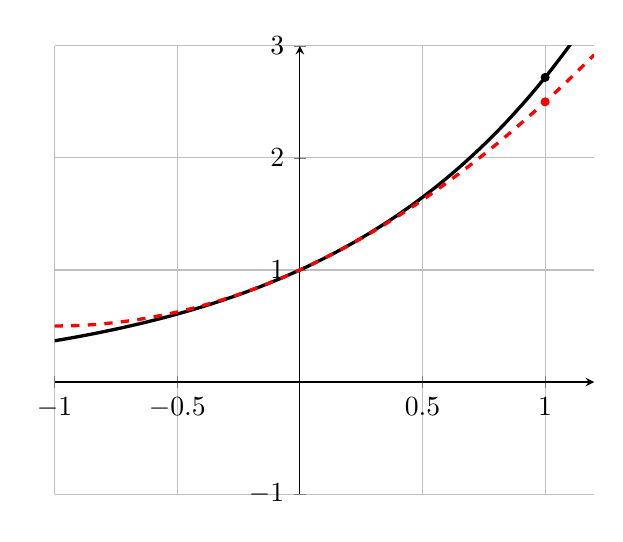
\begin{tikzpicture}
            \begin{axis}[axis lines=center, domain=-1:1.2, xmin=-1, xmax=1.2, ymin=-1, ymax=3,
                grid, legend pos=outer north east]
                \addplot[smooth, black, very thick] {exp(x)};
%                 \addlegendentry{$f(x) = e^x$};
                \addplot[smooth, red, dashed, very thick] {1+x+x^2/2};
%                 \addlegendentry{$g(x) = 1+x+x^2/2$};
                \draw[fill=black] (axis cs:1,2.718282) circle(0.05cm);
                \draw[color=red, fill=red] (axis cs:1,2.5) circle(0.05cm);
            \end{axis}
        \end{tikzpicture}
        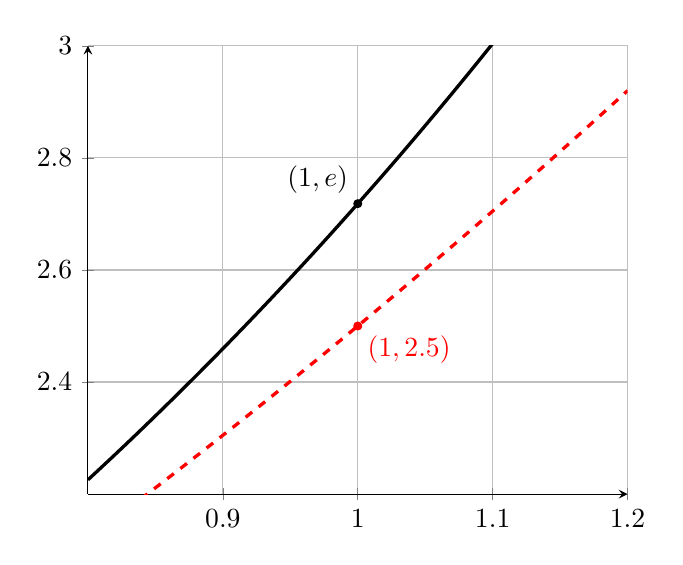
\begin{tikzpicture}
            \begin{axis}[axis lines=center, domain=0.8:1.2, xmin=0.8, xmax=1.2, ymin=2.2, ymax=3,
                grid]
                \addplot[smooth, black, very thick] {exp(x)};
%                 \addlegendentry{$f(x) = e^x$};
                \addplot[smooth, red, dashed, very thick] {1+x+x^2/2};
%                 \addlegendentry{$g(x) = 1+x+x^2/2$};
                \draw[fill=black] (axis cs:1,2.718282) circle(0.05cm);
                \draw[color=red, fill=red] (axis cs:1,2.5) circle(0.05cm);
%                 \draw[blue, thick, dashed] (axis cs:1.1,2.6) -- (axis cs:1,2.71828);
%                 \draw[blue, thick, dashed] (axis cs:1.1,2.6)
%                 node[anchor=west]{$\approx0.218$} -- (axis cs:1,2.5);
                \draw[red] (axis cs:1,2.5) node[anchor=north west]{$(1,2.5)$};
                \draw[black] (axis cs:1,2.71828) node[anchor=south east]{$(1,e)$};
            \end{axis}
        \end{tikzpicture}
    \end{center}
    \caption{The function $f(x) = e^x$ and a second order Taylor approximation. The solid
    black curve is $f(x) = e^x$ and the dashed red curve is the Taylor approximation.  The
right-hand plot shows a zoomed in view near the point $x=1$.}
    \label{fig:taylor_thm_exp}
\end{figure}

\begin{problem}
    The {\it engineer's approximation} to the sine function is:
    \begin{center}
        For $x$ close to $0$, $\sin(x) \approx x$. 
    \end{center}
    Obviously the word {\it close} is relative.  Use Taylor's theorem to determine how
    much error is being made with the {\it engineer's approximation} if you want to calculate $\sin(0.5)$?
    See Figure \ref{fig:taylor_thm_sine}.
\end{problem}
\solution{
    This is simply the first term in the Taylor series, but since the quadratic term is
    zero for the Taylor series for sine we can also think of this as a second order Taylor
    polynomial ($\sin(x) \approx 0 + x + 0x^2$).  Hence, the remainder function is 
    \[ R_3(x) = \frac{f^{(3)}(\xi)}{3!}x^3 \]
    where $\xi$ is some number such that $0 < \xi < 0.5$.  Therefore, $R_3(0.5) =
    \frac{-\cos(\xi)}{6} \cdot (0.125) \approx -0.028 \cos(\xi)$ and since $|\cos(x)|\le
    1$ we know that the error will be less than $0.028$ (approximately) when using the
    engineer's approximation of sine at $0.5$.
}
\begin{figure}[ht!]
    \begin{center}
        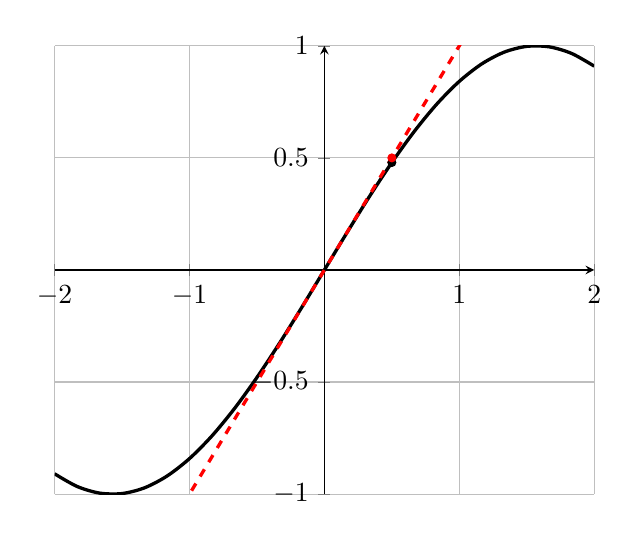
\begin{tikzpicture}
            \begin{axis}[axis lines=center, domain=-2:2, xmin=-2, xmax=2, ymin=-1, ymax=1,
                grid, legend pos=outer north east]
                \addplot[smooth, black, very thick] {sin(deg(x))};
%                 \addlegendentry{$f(x) = e^x$};
                \addplot[smooth, red, dashed, very thick] {x};
%                 \addlegendentry{$g(x) = 1+x+x^2/2$};
                \draw[fill=black] (axis cs:0.5,0.4794) circle(0.05cm);
                \draw[color=red, fill=red] (axis cs:0.5,0.5) circle(0.05cm);
            \end{axis}
        \end{tikzpicture}
        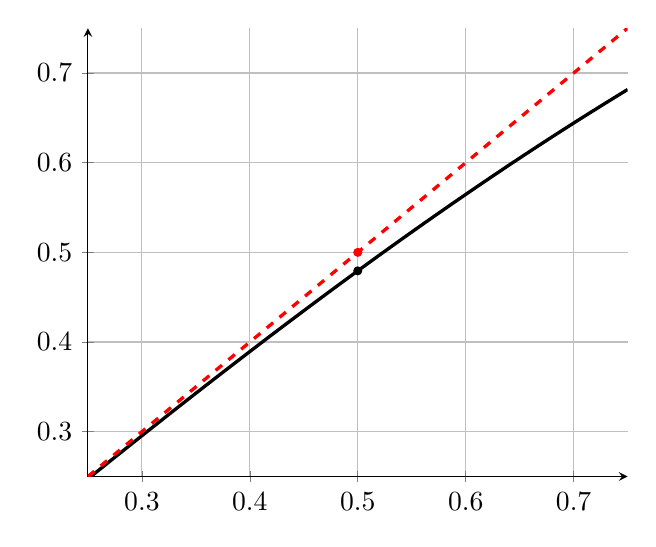
\begin{tikzpicture}
            \begin{axis}[axis lines=center, domain=0.25:0.75, xmin=0.25, xmax=0.75,
                ymin=0.25, ymax=0.75, grid]
                \addplot[smooth, black, very thick] {sin(deg(x))};
%                 \addlegendentry{$f(x) = e^x$};
                \addplot[smooth, red, dashed, very thick] {x};
%                 \addlegendentry{$g(x) = 1+x+x^2/2$};
                \draw[fill=black] (axis cs:0.5,0.4794) circle(0.05cm);
                \draw[color=red, fill=red] (axis cs:0.5,0.5) circle(0.05cm);
            \end{axis}
        \end{tikzpicture}
    \end{center}
    \caption{The function $f(x) = \sin(x)$ and a second order Taylor approximation. The solid
    black curve is $f(x) = \sin(x)$ and the dashed red curve is the Taylor approximation.  The
right-hand plot shows a zoomed in view near the point $x=0.5$.}
    \label{fig:taylor_thm_sine}
\end{figure}


\begin{problem}
    No computational software actually {\it knows} functions like the exponential function
    or the sine function.  Instead, they have a way to calculate values for these
    functions based on Taylor series.  
    If we want to calculate a value for $e^{0.5}$ on a computer, how many terms in the
    Taylor series do we need so that the truncation error is less than machine precision?
\end{problem}
\solution{
    The truncation error for the exponential function is 
    \[ R_n(x) = \frac{e^\xi}{n!} x^n \]
    where $\xi \in (0,0.5)$.  Knowing that the exponential function is
    monotonically increasing we know that $R_n(x) \le \frac{\sqrt{e}}{n!}
    (0.5)^n.$  Hence we can approximate the number of terms by finding $n$
    such that the $\frac{\sqrt{e} 0.5^n}{n!} < 1 \times 10^{-16}$.  Making a table of
    values fo the sequence on the right it is reasonably quick to see that we
    need about 14 or 15 terms in the Taylor series in order for the precision
    of this computation to be less than any observable error on a computer.
}

\begin{example}
    How many terms of the Taylor Series for $e^x$ (centered at $a=0$) are needed to
    calculate $e$ to within 10 decimal places? \\{\bf Solution:} \\
    Recall that if $f(x) = e^x$ then 
    \[ f(x) = \sum_{k=0}^\infty \frac{x^k}{k!}, \]
    and this Taylor Series representation converges for all $x \in \mathbb{R}$.  From
    Taylor's Theorem we know that the remainder term takes the form 
    \[ R_n(x) = \frac{f^{(n+1)}(\xi)}{(n+1)!} x^{n+1} \]
    where $\xi \in (0,1)$. For the exponential function we know that $f^{(n+1)}(\xi) =
    f(\xi) = e^\xi$.  Furthermore, we are trying to approximate the error at $x=1$ so the
    remainder term is 
    \[ R_n(1) = \frac{e^\xi}{(n+1)!}. \]
    We want to find $n$ such that $R_n(1) < 10^{-10}$.  Observe that since $\xi \in (0,1)$
    we know that $e^\xi < e$.  Hence we need $n$ such that $e \cdot 10^{10} < (n+1)!$.
    Examining the orders of magnitude for the factorial sequence we see that $n \ge
    13$ since $(13+1)! \approx 9 \times 10^{10} > e \cdot 10^{10}$.

    Indeed, if we use 13 terms in the Taylor Series for $f(x) = e^x$ we get
    \[ f(1) \approx 2.71828182844676, \]
    and this approximation is correct to the $10^{th}$ decimal digit.
\end{example}

\begin{example}
    Calculate $e$ to within machine precision. \\{\bf Solution:}\\
    Modifying the previous example we see that we need $n$ such that 
    \[ R_n(1) = \frac{e^\xi}{(n+1)!} < 10^{-16}. \]
    Examining the orders of magnitude of the factorial sequence we see that we need $n \ge
    18$ terms in the Taylor Series to have a value of $e$ that is accurate to within
    machine precision.
\end{example}


\newpage\section{Exercises}
Several of the exercises in this section are designed just to get you coding.  If you are
having trouble getting started on the coding please see Appendix \ref{app:MATLAB}.

\begin{problem}
    For each of the following commands tell what the command is asking MATLAB to do and
    why the answer is {\it wrong}.
    \begin{enumerate}
        \item[(a)] \mcode{sqrt(2)^2 == 2}
        \item[(b)] \mcode{(1/49)*49 == 1}
        \item[(c)] \mcode{exp(log(3)) == 3}
    \end{enumerate}
\end{problem}



\begin{problem}
    If we list all of the numbers below 10 that are multiples of 3 or 5 we get 3, 5, 6,
    and 9.  The sum of these multiples is 23.  Write code to find the sum of all the
    multiples of 3 or 5 below 1000.  Your code needs to run error free and output only the
    sum.  Consult some of the examples in Appendix \ref{app:MATLAB} if you're stuck with
    the coding.
\end{problem}
% \solution{
% %     Source: Project Euler Problem \#1: 
% %     Answer: 233,168
% }
\hint{
    Be sure to treat numbers like $15$ carefully.  To find the sum you should have a
    variable in your code that accumulates the running total. 
}


\begin{problem}
    Each new term in the Fibonacci sequence is generated by adding the previous two terms.
    By starting with 1 and 2, the first 10 terms will be:
    \[ 1, 2, 3, 5, 8, 13, 21, 34, 55, 89, \dots \]
    By considering the terms in the Fibonacci sequence whose values do not exceed four
    million, write code to find the sum of the even-valued terms. Your code needs to run
    error free and output only the sum.  Consult some of the examples in Appendix \ref{app:MATLAB} if you're stuck with
    the coding.
\end{problem}
% \solution{
% %     Source: Project Euler Problem \#2: 
% %     Answer: 4,613,732
% }
\hint{
    You probably don't need to store all of the Fibonacci numbers as you go, just the
    current one and the two previous.  To find the sum you should have a
    variable in your code that accumulates the running total.
}

\begin{problem}
    Write computer code that will draw random numbers from the unit interval $[0,1]$,
    distributed uniformly, until
    the sum of the numbers that you draw is greater than 1.  Keep track of how many
    numbers you draw.  Then write a loop that does this process many many times.  On
    average, how many numbers do you have draw until your sum is larger than 1? \\ Hint
    \#1:
    In \texttt{MATLAB} you should use the \mcode{rand(1,1)} command to draw a single
    number from a uniform distribution with bounds $[0,1]$. \\ Hint \#2: You should do
    this more than 1,000,000 times to get a good average \ldots and the number that you
    get should be familiar!
\end{problem}

\begin{problem}
    Use the ratio test to determine the radius of convergence for the functions $\sin(x)$, $\cos(x)$,
    $\ln(1+x)$, and $\arctan(x)$.  Show all of your work and support your answer with
    plots demonstrating your findings graphically.
\end{problem}

\begin{problem}[modified from \cite{Chartier}]
    In the 1999 movie {\it Office Space}, a character creates a program that takes
    fractions of cents that are truncated in a bank's transactions and deposits them to
    his own account.  This is idea has been attempted in the past and now banks
    look for this sort of thing.  In this problem you will build a simulation of the
    program to see how long it takes to become a millionaire.  

    {\bf Assumptions:}
    \begin{itemize}
        \item Assume that you have access to 50,000 bank accounts.
        \item Assume that the account balances are uniformly distributed between
            \$100 and \$100,000.
        \item Assume that the annual interest rate on the accounts is 5\% and the interest
            is compounded daily and added to the accounts, except that fractions of cents
            are truncated.
        \item Assume that your \texttt{illegal} account initially has a \$0 balance.
    \end{itemize}

    {\bf Your Tasks:}
    \begin{enumerate}
        \item[(a)] Explain what the following two lines of MATLAB code do.
% \begin{verbatim}
\begin{lstlisting}
accounts = 100 + (100000-100) * rand(50000,1);
accounts = floor(100*accounts)/100;
\end{lstlisting}
% \end{verbatim}
        \item[(b)] By hand (no computer) write the mathematical steps necessary to
            increase the accounts by (5/365)\% per day, truncate the accounts to the
            nearest penny, and add the truncated amount into an account titled
            ``\texttt{illegal}''.
        \item[(c)] Write code to complete your plan from part (b).
        \item[(d)] Using a \texttt{while} loop, iterate over your code until the illegal
            account has accumulated \$1,000,000.  How long does it take?
    \end{enumerate}
\end{problem}
% Modified from Chartier and Greenbaum, Chapter 5 Problem 14
\hint{
    Be sure that the illegal account is earning interest.
}


\begin{problem}[modified from \cite{Chartier}]
    In the 1991 Gulf War, the Patriot missle defense system failed due to roundoff error.
    The troubles stemmed from a computer that performed the tracking calculations with an
    internal clock whose integer values in tenths of a second were converted to seconds by
    multiplying by a 24-bit binary approximation to $\frac{1}{10}$:
    \[ 0.1_{10} \approx 0.00011001100110011001100_2. \]
    \begin{enumerate}
        \item[(a)] Convert the binary number above to a fraction by hand (common
            denominators would be helpful).
        \item[(b)] The approximation of $\frac{1}{10}$ given above is clearly not equal to
            $\frac{1}{10}$.  What is the absolute error in this value?
        \item[(c)] What is the time error, in seconds, after 100 hours of operation?
        \item[(d)] During the 1991 war, a Scud missile traveled at approximately Mach 5
            (3750 mph).  Find the distance that the Scud missle would travel during the
            time error computed in (c).
    \end{enumerate}
\end{problem}
% Modified from Chartier and Greenbaum, Chapter 5 Problem 15


\begin{problem}[Approximating $\pi$]
    In this problem we will use Taylor Series to build approximations for the irrational
    number $\pi$.
    \begin{enumerate}
        \item[(a)] Write the Taylor series centered at $a=0$ for the function $f(x) =
            \frac{1}{1+x}$.  You may want to refer back to Examples \ref{ex:Taylor1} and
            \ref{ex:Taylor2} to get started.
        \item[(b)] Use the ratio test to determine the domain of convergence for this
            Taylor series.
        \item[(b)] Substitute $t^2$ for $x$ to get a Taylor series for $g(t) =
            \frac{1}{1+t^2}$.
        \item[(c)] Integrate both sides from $t=0$ to $t=y$ to get a Taylor series for
            $h(y) = \arctan(y)$.
        \item[(d)] Use the fact that $\arctan(1) = \pi/4$ along with your answer
            to part (c) to approximate $\pi$ to 10 decimal digits of accuracy.  Use
            Taylor's theorem to prove that you have the correct accuracy.
    \end{enumerate}
\end{problem}
\hint{
    You will need to use Taylor's Theorem to approximate the error and use this to back
    out the number of terms that are necessary.
}

\begin{problem}
    In this problem we will prove the famous (and the author's favorite) formula
    \[ e^{i\theta} = \cos(\theta) + i \sin(\theta). \]
    This is known as Euler's formula after the famous mathematician Leonard Euler.  Show
    all of your work for the following tasks.
    \begin{enumerate}
        \item[(a)] Write the Taylor series for the functions $e^x$, $\sin(x)$, and
            $\cos(x)$.
        \item[(b)] Replace $x$ with $i\theta$ in the Taylor expansion of $e^x$.  Recall
            that $i = \sqrt{-1}$ so $i^2 = -1$, $i^3 = -i$, and $i^4 = 1$.  Simplify all
            of the powers of $i\theta$ that arise in the Taylor expansion.
        \item[(c)] Gather all of the real terms and all of the imaginary terms together.
            Factor the $i$ out of the imaginary terms.  What do you notice?
        \item[(d)] Use your result from part (c) to prove that $e^{i\pi} + 1 =
            0$.
    \end{enumerate}
\end{problem}
\hint{
    \[ e^{i\theta} = 1 + (i\theta) + \frac{(i\theta)^2}{2} + \frac{(i\theta)^3}{3!} +
        \frac{(i\theta)^4}{4!} + \frac{(i\theta)^5}{5!} + \frac{(i\theta)^6}{6!} + \cdots
    \]
}

\begin{problem}
    Create a MATLAB function that accepts an anonymous function handle $f(x)$ and an
    integer $N$ and gives as an output an animation of successive Taylor approximations of
    the function up to the $N^{th}$ term.  \\
    \mcode{function TaylorAnimation(f , N)} \\
    Write a test script that calls your function on several different infinitely
    differentiable functions.  Your test script will look something like the following.
\begin{lstlisting}
clear; clc; clf;
f = @(x) sin(x)
N = 50;
TaylorAnimation(f,N)
\end{lstlisting}
\end{problem}

\begin{problem}[Jenny's Phone Number]
    My favorite prime number is 8675309.  Yep.  Jenny's phone number is prime!  Write a
    MATLAB script that verifies this fact.  You cannot use the built-in MATLAB function
    \mcode{isprime( )}.
    Consult some of the examples in Appendix \ref{app:MATLAB} if you're stuck with
    the coding.
\end{problem}
\hint{
    Remember that a prime number has exactly two divisors: 1 and itself.  
    You only need to check divisors as large as the square root of 8675309 (why). 
}

\begin{problem}
    Write a function called \mcode{MyPrimeChecker} that accepts an integer and returns a
    binary variable: 0 = not prime, 1 = prime.\\
    \mcode{function Primality = MyPrimeChecker(n)} \\
    Next write a MATLAB script to find the sum of all of the prime numbers less than 1000.
    Consult some of the examples in Appendix \ref{app:MATLAB} if you're stuck with
    the coding.
\end{problem}
\hint{
    Remember that a prime number has exactly two divisors: 1 and itself.  
    You only need to check divisors as large as the square root of $n$. Your script should
    probably be smart enough to avoid all of the non-prime even numbers.
}




\begin{problem}
    The sum of the squares of the first ten natural numbers is,
    \[ 1^2 + 2^2 + \dots + 10^2 = 385 \]
    The square of the sum of the first ten natural numbers is,
    \[ (1 + 2 + \dots + 10)^2 = 55^2 = 3025 \]
    Hence the difference between the sum of the squares of the first ten natural numbers
    and the square of the sum is $3025 - 385 = 2640$.

    Write code to find the difference between the sum of the squares of the first one
    hundred natural numbers and the square of the sum.  Your code needs to run error free
    and output only the difference.  
\end{problem}
\hint{
% Source: Project Euler Prolem \#6:
    (big hint) the answer is 25164150. Of course you'll have to write code to get this. 
}

\begin{problem}
    The prime factors of $13195$ are $5, 7, 13$ and $29$.  Write
    code to find the largest prime factor of the number $600851475143$? Your code needs to
    run error free and output only the largest prime factor. 
\end{problem}
\hint{
% Source: Project Euler Problem \#3: 
(big hint) the answer is 6857.  Of course you'll have to write code to get this.}


\begin{problem}
    The number 2520 is the smallest number that can be divided by each of the
    numbers from 1 to 10 without any remainder.  Write code to find the smallest positive
    number that is evenly divisible by all of the numbers from 1 to 20?
\end{problem}
\hint{% Source: Project Euler Problem \#5: 
    Solution: 232792560. You may want to use modular division.  The code \mcode{mod(a,b)}
    will give the remainder when $a$ is divided by $b$.  If the answer is 0 then $a$ can
be divided by $b$.  For example, \mcode{mod(6,2)} is 0 since 6 is divisible by 2, and
\mcode{mod(7,3)} is 1 since 7 divided by 3 is 2 with a remainder of 1.

In this problem you should not be doing an exhaustive search.  
}


\begin{problem}
    The following iterative sequence is defined for the set of
    positive integers:
    \begin{flalign*}
        & n \to \frac{n}{2} \quad \text{(n is even)} \\
        & n \to 3n + 1 \quad \text{(n is odd)}
    \end{flalign*}
    Using the rule above and starting with $13$, we generate the following sequence:
    \[ 13 \to  40 \to 20 \to 10 \to 5 \to 16 \to 8 \to 4 \to 2 \to 1 \]
    It can be seen that this sequence (starting at 13 and finishing at 1) contains 10
    terms. Although it has not been proved yet (Collatz Problem), it is thought that all
    starting numbers finish at 1.

    Write code to determine which starting number, under one million, produces the longest
    chain. NOTE: Once the chain starts the terms are allowed to go above one million.
\end{problem}
% \solution{Source: Project Euler Problem \#14: Solution: 837799}

\begin{problem}
    Find the domain of convergence for the Taylor series for each of the following Taylor
    series.  Center each Taylor series at $a=0$.
    \begin{flalign*}
        f_1(x) &= \sin(x) \\
        f_2(x) &= \cos(x) \\
        f_3(x) &= \frac{1}{1+x} \\
        f_4(x) &= \frac{1}{1-x} \\
        f_5(x) &= \frac{1}{1+x^2} \\
        f_6(x) &= \ln(1+x)
    \end{flalign*}
\end{problem}
